\documentclass[11pt]{article}
\usepackage{fancyheadings,multicol}
\usepackage{amsmath,amssymb,graphicx}


\setlength{\textheight}{\paperheight}
\addtolength{\textheight}{-2in}
\setlength{\topmargin}{-.5in}
\setlength{\headsep}{.5in}
\addtolength{\headsep}{-\headheight}
\setlength{\footskip}{.5in}
\setlength{\textwidth}{\paperwidth}
\addtolength{\textwidth}{-2in}
\setlength{\oddsidemargin}{0in}
\setlength{\evensidemargin}{0in}
\flushbottom

\allowdisplaybreaks

\pagestyle{fancyplain}
\let\headrule=\empty
\let\footrule=\empty
\lhead{\fancyplain{}{Fall 2015}}
\rhead{\fancyplain{}{CSCI-B555: Machine Learning}}
\cfoot{{\thepage/\pageref{EndOfAssignment}}}

\newcounter{totalmarks}
\setcounter{totalmarks}{0}
\newcounter{questionnumber}
\setcounter{questionnumber}{0}
\newcounter{subquestionnumber}[questionnumber]
\setcounter{subquestionnumber}{0}
\renewcommand{\thesubquestionnumber}{(\alph{subquestionnumber})}
\newcommand{\question}[2][]%
  {\ifx\empty#2\empty\else
   \addtocounter{totalmarks}{#2}\refstepcounter{questionnumber}\fi
   \bigskip\noindent\textbf{\Large Question \thequestionnumber. } #1
   {\scshape\ifx\empty#2\empty(continued)\else
   [#2 mark\ifnum #2 > 1 s\fi]\fi}\par
   \medskip\noindent\ignorespaces}
\newcommand{\subquestion}[2][]%
  {\ifx\empty#2\empty\else\refstepcounter{subquestionnumber}\fi
   \medskip\noindent\textbf{\large \thesubquestionnumber } #1
   {\scshape\ifx\empty#2\empty(continued)\else
   [#2 mark\ifnum #2 > 1 s\fi]\fi}
   \smallskip\noindent\ignorespaces}
\newcommand{\bonus}[2][]%
  {\bigskip\noindent\textbf{\Large Bonus. } #1
   {\scshape\ifx\empty#2\empty(continued)\else
   [#2 mark\ifnum #2 > 1 s\fi]\fi}\par
   \medskip\noindent\ignorespaces}

\usepackage{totcount}
\regtotcounter{totalmarks}


\begin{document}

\thispagestyle{plain}

\begin{center}
\bfseries
{\Large Homework Assignment \# 4}\\
   Due: Wednesday, December 9, 2015, 11:59 p.m. \\
   Name: Srijita Das\\
   Email id:sridas@indiana.edu\\
   Total marks: \total{totalmarks}
\end{center}

\question{10}
Use the method of Lagrange multipliers to find extrema of function  $f(x,y)$ under the given constraints.

\subquestion{3}
$f(x,y)=x^2-y^2$ subject to $x^2+y^2=4$

\subquestion{3}
 $f(x,y)=x^2 y-\log x$ subject to  $x+2y=0$
 
 \subquestion{4}
$f(x,y)=x^2+2xy+y^2-2x$ subject to  $x^2-y^2=-1$

Ans: The answers to these problems have been hand written, scanned and uploaded as a separate pdf. Please refer to that.\\


\question{40}
In this question, you will implement kernel linear regression.
Kernel linear regression can be derived using the kernel trick,
where the optimal solution $\mathbf{w} $ is always a function of the training data
$\mathbf{w} = \mathbf{X}^\top \boldsymbol{\alpha}$ for $\mathbf{X}^\top \in \mathbb{R}^{n \times d}$
and $\boldsymbol{\alpha} \in \mathbb{R}^{n}$. Therefore, we could instead learn $\boldsymbol{\alpha}$,
and whenever we predict on a new value $\mathbf{x}$, the prediction is 
$\mathbf{x}^\top \mathbf{w} =  \mathbf{x}^\top \mathbf{X}^\top \boldsymbol{\alpha} = \sum_{i=1}^n k(\mathbf{x}, \mathbf{x}_i) \alpha_i$
with $k(\mathbf{x}, \mathbf{x}_i) = \langle  \mathbf{x}, \mathbf{x}_i \rangle $ in this case. In general, we can extend to other
feature representations on $\mathbf{x}$, giving $\phi(\mathbf{x})$ and so a different kernel $k(\mathbf{x}, \mathbf{x}_i) = \langle \mathbf{x}, \mathbf{x}_i \rangle$.

The kernel trick is useful conceptually, and for algorithm derivation. 
In practice, when implementing kernel regression, we do not need
to consider the kernel trick. Rather, the procedure is simple, involving
replacing your current features with the kernel features and performing standard regression.
For learning, we replace the training data with the new kernel representation:
%
\begin{align*}
\mathbf{K}_{\text{train}} = \left[ \begin{array}{cccc} k(\mathbf{x}_1, \mathbf{c}_1) & k(\mathbf{x}_1, \mathbf{c}_2) & \ldots & k(\mathbf{x}_1, \mathbf{c}_k) \\ 
\vdots & \vdots& \vdots & \vdots \\  
k(\mathbf{x}_n, \mathbf{c}_1) & k(\mathbf{x}_n, \mathbf{c}_2) & \ldots & k(\mathbf{x}_n, \mathbf{c}_k)
  \end{array} \right] 
  \in \mathbb{R}^{n \times k}
\end{align*}
%
for some chosen centers (above those chosen centers were the training data samples $\mathbf{x}_i$). For example,
for the linear kernel above with $k(\mathbf{x}, \mathbf{x}_i) = \langle  \mathbf{x}, \mathbf{x}_i \rangle $, the
center is $\mathbf{c} = \mathbf{x}_i$. Notice that the number of features is now $k$, the number of selected centers,
as opposed to the original dimension $d$. Once your've transformed your data to this new representation,
then you learn $\mathbf{w}$ with linear regression as usual, such that $\mathbf{K}_{\text{train}} \mathbf{w}$
approximates $\mathbf{y}_{\text{train}}$. As before, you can consider adding regularization.
The prediction is similarly simple, where each new point is transformed into a kernel representation using the selected centers. \\

\subquestion{20} 
Implement this algorithm. Run it on the dataset from Assignment2.\\
Ans: I implemented the Kernel Linear Regression in the code attached with the Assignment.A linear kernel is of the form\\
$K(x,y)=x^Ty+C$\\
When I an the Kernel Linear regression on the Blog dataset without doing any regularisation, I got the below results. I ran the data on the Normalized Blog dataset.\\

\begin{tabular}{|c|c|}
\hline 
Method & Error \\ 
\hline 
Linear Regression & 1095.33775337 \\ 
\hline 
Ridge Regression & 1077.20598265 \\ 
\hline 
Random & 373533.45824 \\ 
\hline 
Mean & 1500.01250961 \\ 
\hline 
Kernel Linear Regrssion & 4633.41499249 \\ 
\hline 
\end{tabular} 
\\

My observation is that Kernel Linear Regression does not produce good results without regularisation as I noticed that the weights were increasing. Next, I tried Kernel Linear regression with regularisation of $\alpha=0.1)$. Below jotted down are the results with regularisation aplied to Kernel Linear Regression.\\

\begin{tabular}{|c|c|}
\hline 
Method & Error \\ 
\hline 
Linear Regression & 1.91460361733E+031 \\ 
\hline 
Ridge Regression & 1135.33062632 \\ 
\hline 
Random & 281562.322506 \\ 
\hline 
Mean & 1429.37369207 \\ 
\hline 
Kernel Linear Regrssion & 1135.6070861 \\ 
\hline 
\end{tabular} 
\\

So, with a regularisation parameter of 0.1, Kernel Linear Regression performs better than Random, Mean and Linear Regression but it has the same error as Ridge Regression. Kernel Linear Regression is  not able to outperform ridge Regression.
I even tried doing regularisation with regularisation parameter of 1 and 10 and got error as 1549.86337447 and 1287.69049863. So, it seems that regularisation parameter of 0.1 works best for the case of Kernel Linear Rehression on this dataset. \\

\subquestion{5} 
Explain your implementation choice.\\

Ans:I implemented Kernel Linear Regression with regularisation of 0.1 because that was giving me the best results and performing as good as Ridge Regression. However it could not outperform Ridge Regression with any of the Regularisation parameter. In order to find out the centroids for Kernel linear Regression, I ran k-means clustering with the Python scipy inbuilt package for k-means clustering. The number of centroids considered by me was 400. The maximum number of clusters formed by this algorithm on the Blog dataset is something around 390 to 400. So, I did not increase the number of centroids to more than 400. Also, this datset has around 250 features, so I wanted to keep the number of centroids more than that because kernels perform better in higher dimension. So, after finding the close to 400 centroids by K-means clustering, I applied the linear kernel function to each of the data points for all the 400 centroids. So, the data now got projected to a high dimensional space of dimension 52000 x 400. On this dataset, now I ran Kernel Linear Regression on a random sample of 20000 and a random test sample of 10000 and the results of Kernel Linear Regression are jotted down in part a) of this question.\\ 

\subquestion{15}
Try three different kernels. Explain any difference in behavior on this dataset.\\
Ans: Apart from Linear Kernel, I implemented Gaussian, Laplace and Sigmoid Kernel for this dataset. Since, Linear kernel performed best with regularisation parameter of 0.1, so I used this regularisation parameter for all the three types of Kernel and varied the parameter of the Kernel function to see what the results are.\\

\textbf{Gaussian Kernel:}\\

The function for Gaussian Kernel is as below:\\


$k(x,y)=exp^{\frac{-||x-y||^2}{2\sigma^2}}$
In the above kernel function, the adjustable parameter is $\sigma$ and I varied this parameter across a range of values to see how the Kernel behaves and below jotted down are the results:\\

\begin{tabular}{|c|c|c|c|c|c|}
\hline 
Method & $\sigma=0.01$ & $\sigma=0.1$ & $\sigma=1$ & $\sigma=10$ \\ 
\hline 
Linear Regression & 20477.6247264 & 2405.65694476 & 1515.0216575 & 2379.25518255  \\ 
\hline 
Ridge Regression & 829.80322656 & 1198.4422563 & 1001.97061105 & 1172.80586866  \\ 
\hline 
Random & 373829.368521 & 230263.820186 & 368188.138927 & 671099.924606 \\ 
\hline 
Mean & 1078.58623178 & 1554.19769313 & 1299.12489538 & 1487.68084724 \\ 
\hline 
Kernel Regression & 1078.58623178 & 1554.19776656 & 1299.12532478 & 1487.68087114  \\ 
\hline 
\end{tabular} 
\\

Kernel Regression performs the best with Gaussian Kernel function for a value of $\sigma=0.01$. However, I was able to outperform Linear Regression with the fuirst 10 features selected. But the Gaussian Kernel did as good as the men predictor and I could not outperform or match to Ridge Regression. I guess my choice of $\sigma$ is not that proper. I read up somewhere that overestimating  $\sigma$ leads the Kernel function to behave linearly and underestimating makes it more sensitive to noise in data and decision boundary doesn't become well defined. So, it is quite possible that  the correct choice of $\sigma$ was not made by me. \\

\textbf{Laplace Kernel:}\\

The function for Laplace Kernel is as below:\\

$k(x,y)=exp^{\frac{-||x-y||}{sigma}}$

For this Kernel as well, I kept the regularization parameter fixed at 0.1 and varied the value of $\sigma$ and jotted down the results. The Laplace Kernel is a little less sensitive to the value of $\sigma$ because it contains $\sigma$ in the denominator in place of $\sigma^2$.\\
Below jotted down are the results:\\

\begin{tabular}{|c|c|c|c|c|c|}
\hline 
Method & $\sigma=0.01$ & $\sigma=0.1$ & $\sigma=1$ & $\sigma=10$ &$\sigma=100$ \\ 
\hline 
Linear Regression & 234868.137095 & 2824.18717099 & 1336.90715324 & 6393.51495831 & 1420.3865 \\ 
\hline 
Ridge Regression & 1100.23233898 & 1295.5670394 & 1283.40061208 & 1439.28038306 & 1211.8692\\ 
\hline 
Random & 664118.843534 & 623086.280994 & 669634.797672 & 365250.475236 & 667039.434 \\ 
\hline 
Mean & 1448.70647627 & 1658.79761945 & 1618.70857192 & 1747.11271772 & 1625.10271 \\ 
\hline 
Kernel Linear Regression & 1448.7066488 & 1658.79762626 & 1614.63430587 & 1740.88771105 & 1609.33836 \\ 
\hline 
\end{tabular} 
\\


The Laplace Kernel behave almost similar to the Gaussian Kernel. I couldn't make it outperform Mean predictor. However, it performs as good as mean predictor. It performs well for the value of $\sigma=0.01$ and $\sigma=0.1$. As I increase the value of $\sigma$ further, the error starts getting larger than Mean predictor.\\


\textbf{Hyperbolic Tangent(Sigmoid) Kernel:}\\

The Kernel function for hyperbolic tangent Kernel is as below:\\

$k(x,y)=tanh(\alpha x^T y+c)$\\

The adjustable or varying parameters here is the slope of the line $\alpha$ and the intercept constant c. I took the value of the slope to be $1/N$.THen I tried running the Hyperbolic tan Kernel for various values of C and got the below results:\\

\begin{tabular}{|c|c|c|c|c|c|}
\hline 
Method & c=0.01 & c=0.1 & c=0 & c=1 & c=10 \\ 
\hline 
Linear Regression & 8103.961 & 3028.29813632 & 2535762.41601 & 1897.76773657 & 5002.40479 \\ 
\hline 
Ridge Regression & 968.00392339 & 1004.60024942 & 1570.54065718 & 1593.65444629 & 1219.902517 \\ 
\hline 
Random & 620949 & 662214.63149 & 670548.098603 & 678969.803707 & 248283.2949 \\ 
\hline 
Mean & 1295.413 & 1246.19626161 & 1858.34169856 & 2017.93715696 & 1495.467714 \\ 
\hline 
Kernel linear Regression & 1295.413 & 1342.84346345 & 1803.68109981 & 1739.38672574 & 1495.467714 \\ 
\hline 
\end{tabular} \\


I did not notice a significant difference than Gaussian and Laplace kernel while implementing hyperbolic tangent Kernel. It performs almost as good as Mean predictor and I cannot outperform or equalize Ridge Regression. However, for C=1, I was able to outperform Mean predictor with an error of 1739 and it was performing pretty close to Mean Predictor.\\

Code for this part has been attached with the Assignment.\\


\question{50}
Take two methods from the last assignment, that you implemented, and run them on a single dataset, the SUSY dataset.
Proper comparisons should be made using 10-fold cross-validation experiments. Use your knowledge about model comparison to formally conclude which of the two algorithms is better. This includes proper training-test splits, statistical significance tests, and proper meta-parameter selection techniques (e.g., cross-validation). You can use statistical significance tests built-in to python (or other languages). Provide a precise conclusion of your experiment. \\

Ans: The sussy dataset contains 100000 data points in total. In my experiment, I randomly resampled a random training set of size 20000 and test set of size 10000 40 times and took the accuracy readings for 40 runs. For each of these runs for three algorithms: Naive Bayes, Logistic Regression and Neural Network, I did a 10-fold cross validation on each of these randomly picked 20000 data points of training. Each fold of my 10-fold cross validation had random data points picked. For Logistic Regression, I varied the regularization parameter. I tried the the following regularisation parameter for Logistic Regression:0.0001,0.001,0.01,0.1,0,1,10,100,1000 and 10000. For Neural Network, the parameter is the number of hidden nodes for the single hidden layer model that we implemented. I tried out the following values for number of hidden nodes:40,48,64,80,96,112,128,144,160,176,192. For each of these parameters, I ran the 10- fold cross validation of each of the parameters and then I chose the parameter of the model that gave the highest accuracy. Using this parameter of the model as the best parameter, I then ran these algorithms( Logistic Regression and Neural Network) on the entire training set of 20000. After learning the model on the entire training set with the best parameters accross all the 10-folds, I then used this model to predict the test set of 10000. The accuracy that came for Logistic Regression, Naive Bayes and Neural Network was then collected for 40 runs of the entire procedure described above. For each of these 40 runs, the models were allowed to choose the best parameters when ran over all the 10 folds and then this best parameter was used to learn the model on the entire training data.
Below is the list of 10 accuracies I collected for the three algorithms. The other 30 accuracy readings have been collected but not mentioned in the assignment.\\

\begin{tabular}{|c|c|c|}
  \hline 
  Neural Network & Logistic Regression & Naive Bayes \\ 
  \hline 
  77.14 & 76.48 & 73.58 \\ 
  \hline 
  78.05 & 76.82 & 74.58 \\ 
  \hline 
  76.45 & 76.23& 73.84\\ 
  \hline 
  77.85 & 76.78 & 74.67 \\ 
  \hline 
  78.2 & 76.61 & 73.64 \\ 
  \hline 
  76.24 & 76.26 & 73.98 \\ 
  \hline 
  76.92 & 76.61 & 74.48 \\ 
  \hline 
  75.73 & 75.92 & 73.45 \\ 
  \hline 
  63.41 & 76.19 & 73.74 \\ 
  \hline 
  77.59 & 77.31 & 74.61 \\ 
  \hline 
  \end{tabular}\\
  
  Now, with these 40 accuracy readings, I performed t-tests in R between accuracy readings of each pair of these algorithms. In order to see whether significant difference exists between these algorithms, I first created the boxplot of the accuracies as in Figure~\ref{Boxplot of Accuracies}. Next, I used qqplot to see if the accuracy measurements follows normal distribution as seen in Figure ~\ref{Logistic qqplot},\ref{Bayes qqplot},\ref{Neural qqplot}. The accuracy measurements of the three algorithms follow a somewhat normal distribution.\\
  
\label{section: Boxplot of Accuracies}
\quad
\begin{figure}[h]
  \begin{center}
    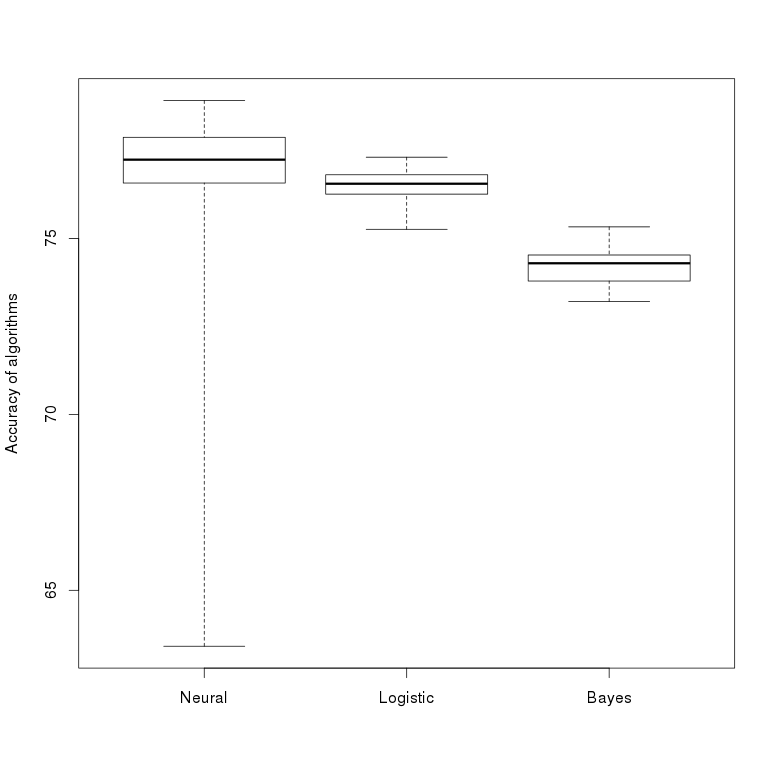
\includegraphics[scale=0.30]{Accuracy_algos.png}
  \end{center}
  \caption{Boxplot of accuracies}
  \label{Boxplot of Accuracies}
\end{figure}
\quad

\label{section: Neural qqplot}
\quad
\begin{figure}[h]
  \begin{center}
    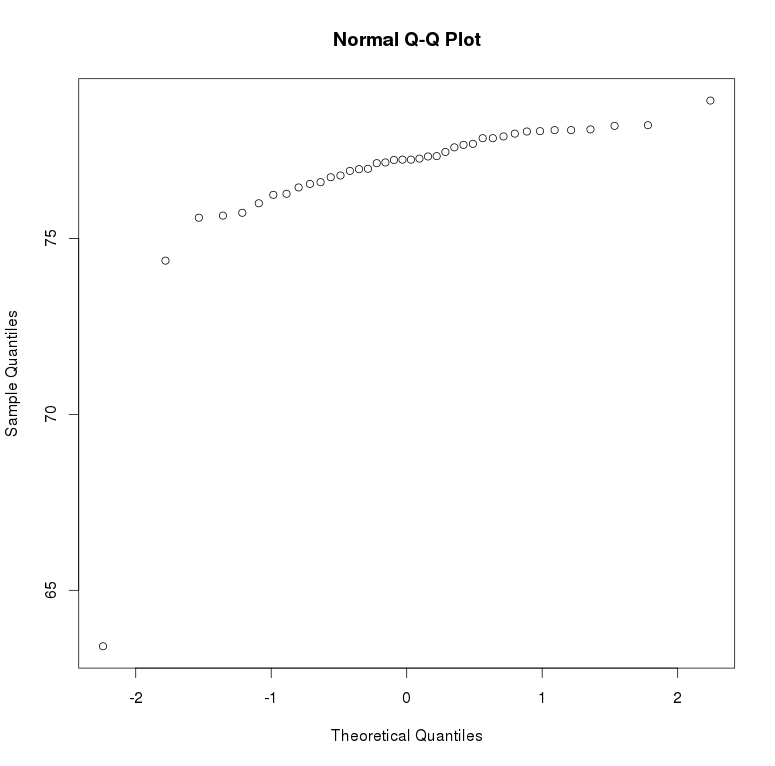
\includegraphics[scale=0.30]{Neural.png}
  \end{center}
  \caption{Neural qqplot}
  \label{Neural qqplot}
\end{figure}
\quad

\label{section: Logistic qqplot}
\quad
\begin{figure}[h]
  \begin{center}
    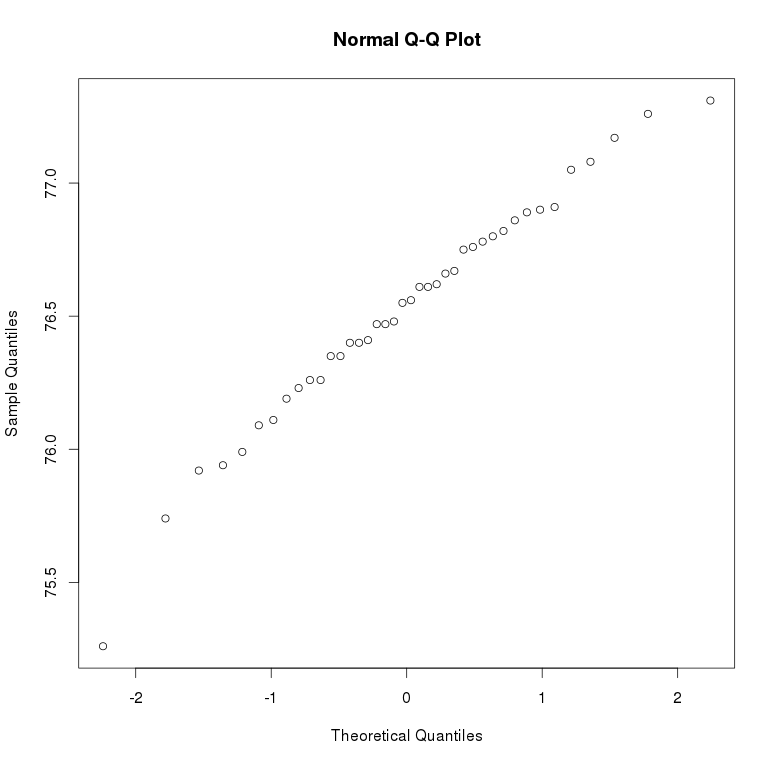
\includegraphics[scale=0.30]{Logistic.png}
  \end{center}
  \caption{Logistic qqplot}
  \label{Logistic qqplot}
\end{figure}
\quad

\label{section: Bayes qqplot}
\quad
\begin{figure}[h]
  \begin{center}
    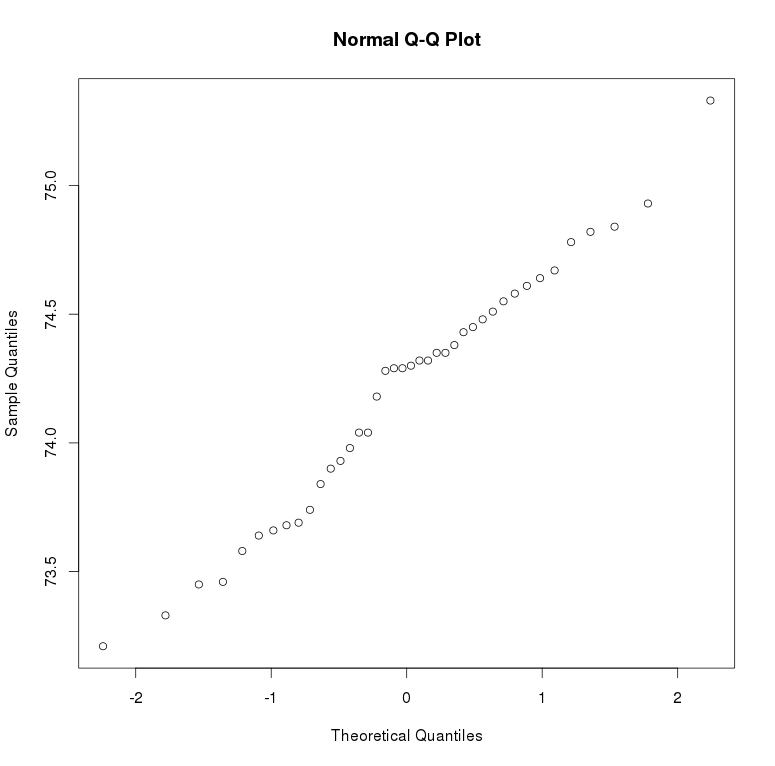
\includegraphics[scale=0.30]{Bayes.png}
  \end{center}
  \caption{Bayes qqplot}
  \label{Bayes qqplot}
\end{figure}
\quad

The output for the t-test and R-code is as below:\\
\begin{verbatim}
Neural.acc = data1[data1$Algos=="Neural"]
Logistic.acc = data1[data1$Algos=="Logistic"]
Bayes.acc = data1[data1$Algos=="Bayes"]

anova(lm(Accuracy ~ Algo, data=data2))

Analysis of Variance Table

Response: Accuracy
           Df Sum Sq Mean Sq F value    Pr(>F)    
Algo        2 165.33  82.665  41.599 2.256e-14 ***
Residuals 117 232.50   1.987                      
---
Signif. codes:  0 ?***? 0.001 ?**? 0.01 ?*? 0.05 ?.? 0.1 ? ? 1

#########T-test for comparing the algorithms
t.test(Neural.acc,Logistic.acc,alternative="greater")

	Welch Two Sample t-test

data:  Neural.acc and Logistic.acc
t = 0.78896, df = 41.564, p-value = 0.2173
alternative hypothesis: true difference in means is greater than 0
95 percent confidence interval:
 -0.3380138        Inf
sample estimates:
mean of x mean of y 
  76.8220   76.5235 
  
t.test(Neural.acc,Bayes.acc,alternative="greater")

	Welch Two Sample t-test

data:  Neural.acc and Bayes.acc
t = 6.908, df = 42.309, p-value = 9.483e-09
alternative hypothesis: true difference in means is greater than 0
95 percent confidence interval:
 1.986543      Inf
sample estimates:
mean of x mean of y 
 76.82200  74.19625 
 
t.test(Logistic.acc,Bayes.acc,alternative="greater")

	Welch Two Sample t-test

data:  Logistic.acc and Bayes.acc
t = 22.765, df = 76.757, p-value < 2.2e-16
alternative hypothesis: true difference in means is greater than 0
95 percent confidence interval:
 2.157043      Inf
sample estimates:
mean of x mean of y 
 76.52350  74.19625
 
\end{verbatim}  

First, I did ANOVA test to see if there was any difference in means between these 3 groups. The p-value of f statistic is very less which suggested that there exists difference in means between any pair of groups. Then, I carried out pairwise t-tests between the accuracy measurements of Logistic Regression, Neural Network and Naive Bayes.Neural Network and Logistic Regression had no statistically significant difference in accuracy measurements with the p-value being 0.2.When I compared, Neural network and Naive Bayes, there exists a statistically significant difference in their accuracy  with the p-value being very less. However, the 95\% confidence interval ranges from 1.98 to infinity which weakens the fact that statistically significant differences exist. We cannot assert this with huge confidence because of this extremely wide confidence interval. Similarly, when I compare Logistic Regression nd Naive Bayes, p-value is very small but the confidence interval is too wide(2.15 to infinity) thus making it difficult to make any statistically significant claims.\\

Thus, I would say that for this particular dataset, no statistically significant difference exists between the accuracies of these three algorithms. The code for this experiment is attached with the submission made. 
\vspace{0.5cm}
\begin{center}
{\large \textbf{Homework policies:}}
\end{center}
Your assignment will be submitted as a single pdf document and a zip file with code, on canvas. 
The questions must be typed; for example, in Latex, Microsoft Word, Lyx, etc.
or must be written legibly and scanned.
Images may be scanned and inserted into the document if it is too complicated to draw them properly. 
%Submit a single pdf document or, if you are attaching your code, 
%submit your code together with the typed (single) document as one .zip file.
%
All code (if applicable) should be turned in when you submit your assignment. 
Use Matlab, Python, R, Java or C.
Policy for late submission assignments: Unless there are legitimate circumstances, late assignments will be accepted up to 5 days after the due date and graded using the following rule: 
\begin{enumerate}
\itemsep0em 
\item[]    on time:	your score � 1
 \item[]   1 day late: 	your score � 0.9
\item[]    2 days late: 	your score � 0.7
\item[]    3 days late: 	your score � 0.5
 \item[]   4 days late: 	your score � 0.3
 \item[]   5 days late: 	your score � 0.1
\end{enumerate}
For example, this means that if you submit 3 days late and get 80 points for your answers, your total number of points will be $80 \times 0.5 = 40$ points.
All assignments are individual, except when collaboration is explicitly allowed. All the sources used for problem solution must be acknowledged, e.g. web sites, books, research papers, personal communication with people, etc. Academic honesty is taken seriously; for detailed information see Indiana University Code of Student Rights, Responsibilities, and Conduct.
\begin{center}
{\large \textbf{Good luck!}}
\end{center}

\label{EndOfAssignment}%

\end{document}
